\documentclass[10pt,twocolumn,a4paper]{article}

% ── Page and type ────────────────────────────────────────────────────
\usepackage[a4paper,margin=0.75in,columnsep=0.3in,top=0.85in,bottom=0.9in]{geometry}
\usepackage[T1]{fontenc}
\usepackage[utf8]{inputenc}
\usepackage{newtxtext,newtxmath}
\usepackage[varqu,varl,scaled=0.95]{inconsolata}
\usepackage[protrusion=true,expansion=true]{microtype}
\usepackage{xcolor}
\usepackage{booktabs,multirow,tabularx,colortbl,array}
\usepackage{enumitem}
\usepackage{caption}
\usepackage{float}
\usepackage{ragged2e}
\usepackage{listings}
\usepackage{tikz}
\usetikzlibrary{positioning,arrows.meta,fit,backgrounds,calc,shapes.geometric}
\usepackage{titlesec}
\usepackage{fancyhdr}
\usepackage[numbers,sort&compress]{natbib}
\usepackage{xurl}
\usepackage[hidelinks,pdfusetitle]{hyperref}
\usepackage[capitalise,noabbrev]{cleveref}

\definecolor{ink}{HTML}{1F2933}
\definecolor{accent}{HTML}{1B5E8C}
\definecolor{soft}{HTML}{EEF3F7}
\definecolor{warn}{HTML}{9C3D10}
\definecolor{rule}{HTML}{9AA5B1}
\color{ink}

\hypersetup{colorlinks=true,linkcolor=accent,citecolor=accent,urlcolor=accent}

\titleformat{\section}{\normalfont\large\bfseries\color{accent}}{\thesection}{0.6em}{}
\titleformat{\subsection}{\normalfont\normalsize\bfseries}{\thesubsection}{0.5em}{}
\titleformat{\paragraph}[runin]{\normalfont\normalsize\bfseries}{}{0pt}{}[.]
\titlespacing*{\section}{0pt}{1.4ex plus .4ex minus .2ex}{0.8ex plus .2ex}
\titlespacing*{\subsection}{0pt}{1.1ex plus .3ex minus .2ex}{0.5ex plus .1ex}
\titlespacing*{\paragraph}{0pt}{0.7ex plus .2ex minus .1ex}{0.6em}

\captionsetup{font=small,labelfont={bf,color=accent},labelsep=period,skip=4pt}
\setlist{nosep,leftmargin=1.2em}
\setlength{\parskip}{0pt}
\renewcommand{\arraystretch}{1.12}

\lstset{basicstyle=\ttfamily\footnotesize,columns=fullflexible,keepspaces=true,
  frame=single,rulecolor=\color{rule},backgroundcolor=\color{soft},
  xleftmargin=3pt,xrightmargin=3pt,aboveskip=6pt,belowskip=4pt,
  breaklines=true,showstringspaces=false}

\newcommand{\code}[1]{\texttt{\small #1}}
\newcommand{\file}[1]{\texttt{\small\color{accent!70!ink}#1}}
\newcommand{\sys}{DecentAI}
\newcommand{\eg}{e.g.,\ }
\newcommand{\ie}{i.e.,\ }

\pagestyle{fancy}
\fancyhf{}
\renewcommand{\headrulewidth}{0pt}
\fancyfoot[C]{\small\thepage}
\fancyhead[R]{\small\color{rule}\sys: A Secure Operating System for AI Agents}
\fancypagestyle{plain}{\fancyhf{}\fancyfoot[C]{\small\thepage}}

\title{\vspace{-1.2em}\Large\bfseries\color{accent}
  DecentAI: A Secure Operating System for AI Agents\\[0.35em]
  \large\mdseries\itshape\color{ink} The model proposes; the platform disposes}
\author{\normalsize Ahmed Dirir\\[0.1em]
  \small DecentAI\\
  \small\href{mailto:ahmed@decentai.io}{\texttt{ahmed@decentai.io}}}
\date{\small October 2026}

\begin{document}

\twocolumn[
\begin{@twocolumnfalse}
\maketitle
\thispagestyle{plain}
\begin{center}
\begin{minipage}{0.86\textwidth}
\small
\noindent\textbf{\color{accent}Abstract.}
Large language models are increasingly used not only to answer but to
act: to send mail, edit records, browse, and run code on a person's
behalf. The models that plan these actions state falsehoods with
confidence and follow instructions embedded in what they read, and the
tools they invoke are third-party code. We present \sys{}, a
self-hosted platform for AI agents built on a single principle: the
model may propose any action, but holds no authority to perform one.
Every proposal is a structured request that passes through gates the
model cannot read or influence---deny-by-default access control with
two machine-checked invariants, a per-call executor that holds each
agent to a manifest approved before its code runs, a person-chosen
trust level with approvals bound to the exact call by hash, and a
layered sandbox (a uid per agent, Landlock, a seccomp denylist, and an
egress proxy that admits only declared hosts). Credentials are
decrypted by the backend and lent to one agent for one call, never to
the model; what is displayed as data beside the model's words is
rendered from stored, schema-validated results of real calls rather
than from the model's text. The design applies operating-system ideas
to agents: processes, users, system calls, a firewall, a scheduler,
kill, and an append-only log. We describe the threat model, each
mechanism with the code that implements it, and an evaluation through
more than two thousand automated tests---including a deliberately
hostile agent that attempts each known escape---and we state every
limit we know of, including those the design accepts on purpose.
\end{minipage}
\end{center}

\vspace{1.4em}
\end{@twocolumnfalse}
]

\section{Introduction}
\label{sec:intro}

An assistant that only talks can be wrong in one way: it says
something false, and a person reads it. An assistant that \emph{acts}
is different. Consider the request that runs through this paper:

\begin{quote}\itshape
``Email the three customers whose invoices are overdue, and remind me
on Friday if any of them hasn't paid.''
\end{quote}

\noindent Carrying it out means reading a spreadsheet, opening a
mailbox, writing three messages, sending them under the person's name,
and acting again on Friday. Each step is an act in the world, and a
sent email cannot be recalled. The properties that make a language
model useful for this---it reads anything, writes fluently, and fills
gaps on its own---are the properties that make it dangerous to hold
the keys.

Five failures follow. A model \emph{fabricates}: ``I've sent the three
reminders'' is a sentence it can produce whether or not any mail left.
It is \emph{steered by what it reads}: text inside a document or an
email can pose as instructions, and no reliable defence against this
\emph{prompt injection} exists inside the model
itself~\cite{greshake2023indirect,perez2022ignore}. Given a person's
credentials, it \emph{oversteps}, because nothing stands between a
mistaken idea and its consequence. It \emph{leaves no trace} other than
its own account of what it did. And its tools are \emph{strangers'
code}, with their own dependencies, any of which may be careless or
hostile.

\paragraph{Approach}
\sys{} does not try to make the model trustworthy. It removes the
model from every decision that matters:

\begin{center}
\emph{The model may propose anything. It decides nothing.}
\end{center}

\noindent The model emits one structured action at a time---call this
function with these inputs, show this stored result, set this
reminder. Whether that action happens is decided by the platform: from
who the person is, what the chat permits, what the agent declared
before it was approved, and what the person approved, in code the
model cannot read, change, or argue with. None of these inputs is
derived from model output, so injected text can steer what the model
\emph{proposes} but cannot widen what may \emph{run}.

The design is deliberately unoriginal in its parts. It applies the
oldest ideas in operating systems~\cite{saltzer1975protection,
anderson1972planning} to a new kind of program: each agent is a
process running as its own user, its requests are system calls that
may be refused, its network access passes through a firewall, risky
actions ask the person first, a scheduler runs deferred work, a kill
switch ends what runs, and a log records what happened. What is new is
the component no operating system was designed for: a planner that is
highly capable and not trusted.

\paragraph{Contributions}
This paper makes the following contributions.

\begin{enumerate}[label=(\arabic*),leftmargin=1.6em]
\item A \textbf{separation of proposal from authority} for LLM agents,
  in which the model holds no permission, credential, or secret, and
  every proposed action is validated and gated by mechanisms none of
  whose inputs derive from model output (\cref{sec:design,sec:execution}).
\item A \textbf{deny-by-default authorization model} with two
  invariants checked on every change---an organization cannot lock
  itself out, and nobody can grant what they do not hold---and a
  \textbf{delegation} scheme under which the agent runtime acts for a
  person only through a short-lived, chat-bound, opaque token fenced to
  a fixed list of 40 actions (\cref{sec:authority}).
\item An \textbf{executor with call-bound approval}: an ordered
  sequence of gates on every function call, a person-chosen trust
  level, and approvals bound to the exact call by a hash that survives
  process restarts and is re-checked against current grants
  (\cref{sec:execution}).
\item \textbf{Evidence by construction}: anything displayed as data
  beside the model's words---tables, charts, files, ``verified''
  marks---is rendered from stored results of successful, schema-validated
  calls, never from the model's text (\cref{sec:evidence}).
\item A \textbf{manifest-first agent model}: each agent declares its
  functions, schemas, permission levels, resources, credential shapes,
  and network hosts before approval; approval pins one commit and one
  content-addressed package; and every call is held to the manifest
  (\cref{sec:agents}).
\item A \textbf{layered, self-inspecting sandbox} for untrusted agent
  code that needs no user namespaces: a capability-bearing spawn helper
  applies resource limits, \code{no\_new\_privs}, a per-agent uid, a
  Landlock ruleset and a seccomp denylist, behind an egress proxy and
  an nftables rule keyed on socket owner; the platform refuses to start
  where it cannot confine and reports what is not enforced where it
  runs (\cref{sec:sandbox}).
\item A \textbf{complete, open implementation} and an evaluation by
  more than two thousand automated tests, including a deliberately
  hostile agent, together with an explicit catalogue of limits
  (\cref{sec:implementation,sec:evaluation,sec:limitations}).
\end{enumerate}

\paragraph{What this paper does not claim}
\sys{} does not make a model correct, does not detect prompt injection,
and does not prevent an agent from misusing what it was rightly given.
Its claims are about containment and visibility: a mistake can lead
only to a call the person was already allowed to make, through an
agent the organization approved, reaching only declared places, with
anything above the chat's trust level waiting for the person's yes;
and every such call is recorded. \Cref{sec:limitations} lists where
these claims are weaker than they sound.

\paragraph{Organization}
\Cref{sec:threat} states the threat model. \Cref{sec:design} gives the
design and follows the running example end to end.
\Cref{sec:authority,sec:execution,sec:evidence,sec:agents,sec:sandbox,sec:secrets,sec:control}
describe each mechanism, naming the source files that implement it.
\Cref{sec:implementation} describes the implementation,
\cref{sec:evaluation} the evaluation, and \cref{sec:limitations} the
limits.

\section{Threat Model and Goals}
\label{sec:threat}

\sys{} is deployed as one instance per organization, on the
organization's own machines, as a set of containers. One instance may
host several organizations (tenants). People use it through a web or
mobile app; scripts use API keys; outside systems may post events to
webhooks.

\paragraph{Assets}
\Cref{tab:assets} lists what is protected and where it lives. The
central decision is that the most valuable assets---the database and
the keys that decrypt it---are held by one component, the backend, and
by nothing that runs untrusted code or talks to the model.

\begin{table}[t]
\centering\small
\caption{Assets and where they are held.}
\label{tab:assets}
\begin{tabularx}{\columnwidth}{@{}>{\raggedright\arraybackslash}p{0.27\columnwidth}>{\raggedright\arraybackslash}X@{}}
\toprule
\textbf{Asset} & \textbf{Held by (and never by)} \\
\midrule
Database contents & the database container, reachable only by the backend on an internal network (not the runtime, not agents) \\
Encryption and signing keys & the backend only \\
A decrypted credential & the backend; the runtime, for one call; the worker of the agent it was lent to (never the model, never the app) \\
A model provider key & the backend; the runtime in memory (never agent code: an agent asks the runtime to call the model for it) \\
The audit trail & an append-only store the API exposes no way to edit \\
\bottomrule
\end{tabularx}
\end{table}

\paragraph{Adversaries}
We consider six.
\begin{enumerate}[label=A\arabic*.,leftmargin=2em]
\item \emph{The model}, not hostile but wrong in unpredictable ways. It
  can emit any action the vocabulary allows, with any inputs, and write
  any prose.
\item \emph{An injector}: anyone who can place text before the
  model---the author of an email, a web page, an uploaded document, an
  agent's result, or a webhook's posted fields. The injector cannot
  touch the platform; it can only hope the model obeys.
\item \emph{An agent's author}, and the author of every dependency. Once
  an agent is approved, its code runs on the platform's machine and,
  during a call, holds what the call was handed; because a worker
  process is kept warm between calls, it could retain it.
\item \emph{Another person}, in the same organization or another.
\item \emph{A compromised worker} that attacks the container's other
  tenants.
\item \emph{A compromised runtime}: the component that runs the
  assistant loop and the agents' executor, taken over through an
  escape from a worker or a flaw of its own.
\end{enumerate}

\paragraph{Out of scope}
We do not defend against (i)~an organization administrator acting in
bad faith: they are the source of the authority the platform enforces;
(ii)~the deployment operator, who holds the database and its keys;
(iii)~the kernel, container engine and hardware, which every container
shares---the seccomp filter narrows the reachable kernel surface but
does not remove the dependence; (iv)~the model provider, to which the
transcript, including function results, is sent when a hosted model is
used; and (v)~a person approving a call they did not read. Denial of
service by an authorized person is bounded only where stated.

\paragraph{Goals}
Against A1--A6 the platform aims to provide:
\begin{enumerate}[label=G\arabic*.,leftmargin=2em]
\item \emph{No authority from words.} Whether an action may run is
  determined from identity, grants, the chat's trust level, the agent's
  approved manifest, and the person's explicit approval; no input to
  that decision is derived from model output.
\item \emph{Containment.} The most a proposal can lead to is a call
  the person could already make, through an approved agent, reaching
  only declared hosts; a call above the chat's trust level waits for
  the person's approval of that exact call.
\item \emph{Faithful display.} What is shown as data beside the model's
  words comes from stored results of real calls.
\item \emph{Confinement.} An agent's code reads and writes only its own
  files, runs as its own user, reaches only declared hosts, uses bounded
  resources, and cannot make the system calls container escapes begin
  with.
\item \emph{Credential isolation.} A credential reaches only the agent
  it was lent to, for the call that needs it, and never the model.
\item \emph{Control and accountability.} A stop ends what runs and
  holds until the person lifts it; actions are recorded on a trail the
  platform only appends to.
\item \emph{Small blast radius.} Each component holds as little as its
  job needs, so compromising one gains as little as possible.
\end{enumerate}

\section{Design}
\label{sec:design}

\subsection{An operating system for agents}

\Cref{tab:os} maps the familiar mechanisms of an operating system onto
\sys{}. The analogy holds where the table says it does and no further:
\sys{} is not a kernel. It runs on Linux in containers and borrows the
kernel's own protections (\cref{sec:sandbox}).

\begin{table}[t]
\centering\small
\caption{Operating-system mechanisms and their counterparts.}
\label{tab:os}
\begin{tabularx}{\columnwidth}{@{}>{\raggedright\arraybackslash}p{0.36\columnwidth}>{\raggedright\arraybackslash}X@{}}
\toprule
\textbf{Operating system} & \textbf{\sys{}} \\
\midrule
installed program and its permissions & \emph{agent} and its \emph{manifest}, reviewed before approval \\
process & \emph{worker}: the one process an approved agent's code runs in \\
user account, file permissions & a uid per agent, and a Landlock fence on its files \\
system call & \emph{function call} through the executor's gates; the worker's own system calls are filtered too \\
firewall & the egress \emph{proxy}, open only to declared hosts \\
``allow this app to\ldots?'' & an \emph{approval card} for one exact call \\
scheduler & the chat's \emph{clock} \\
kill & \emph{stop}, and a per-person stop-everything switch \\
system log & the append-only \emph{audit trail} \\
\bottomrule
\end{tabularx}
\end{table}

\subsection{Components and trust}

\Cref{fig:arch} shows the deployment. Each component is trusted with
something and with nothing more than it needs.

\begin{figure*}[t]
\centering
\resizebox{\textwidth}{!}{%
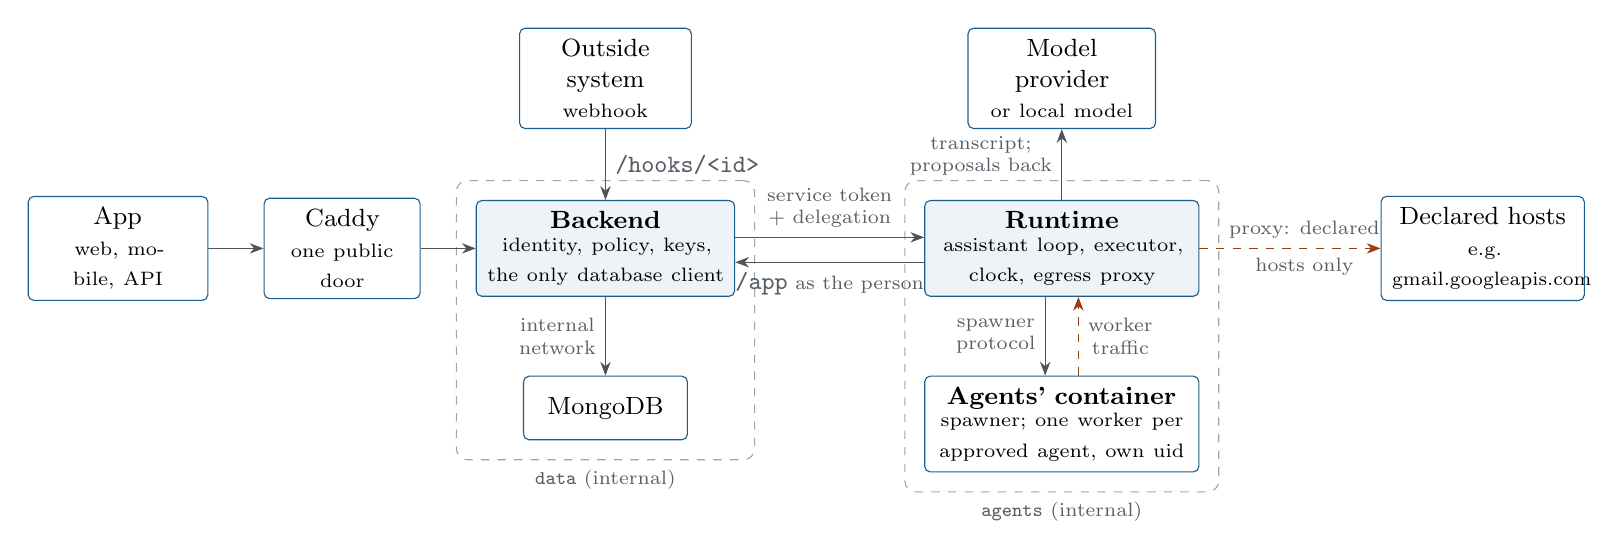
\begin{tikzpicture}[
  font=\small,
  box/.style={draw=accent,rounded corners=2pt,fill=white,minimum height=2.3em,
              align=center,inner sep=4pt,text width=#1},
  box/.default=2.6cm,
  net/.style={draw=rule,dashed,rounded corners=4pt,inner sep=7pt},
  arr/.style={-{Stealth[length=5pt]},draw=ink!80},
  dar/.style={-{Stealth[length=5pt]},draw=warn,dashed},
  lab/.style={font=\scriptsize,text=ink!75,align=center}]
  \node[box=2.0cm] (app) {App\\{\scriptsize web, mobile, API}};
  \node[box=1.7cm,right=0.7cm of app] (caddy) {Caddy\\{\scriptsize one public door}};
  \node[box=3.0cm,right=0.7cm of caddy,fill=soft] (backend) {\textbf{Backend}\\{\scriptsize identity, policy, keys,\\the only database client}};
  \node[box=1.8cm,below=1.0cm of backend] (db) {MongoDB};
  \node[box=3.2cm,right=2.4cm of backend,fill=soft] (runtime) {\textbf{Runtime}\\{\scriptsize assistant loop, executor,\\clock, egress proxy}};
  \node[box=2.1cm,above=0.9cm of runtime] (llm) {Model provider\\{\scriptsize or local model}};
  \node[box=3.2cm,below=1.0cm of runtime] (agents) {\textbf{Agents' container}\\{\scriptsize spawner; one worker per\\approved agent, own uid}};
  \node[box=2.3cm,right=2.3cm of runtime] (inet) {Declared hosts\\{\scriptsize e.g.\ gmail.googleapis.com}};
  \node[box=1.9cm,above=0.9cm of backend] (hook) {Outside system\\{\scriptsize webhook}};

  \draw[arr] (app) -- (caddy);
  \draw[arr] (caddy) -- (backend);
  \draw[arr] (hook) -- node[lab,right]{\code{/hooks/<id>}} (backend);
  \draw[arr] (backend) -- node[lab,left]{internal\\network} (db);
  \draw[arr] ([yshift=4pt]backend.east) -- node[lab,above]{service token\\+ delegation} ([yshift=4pt]runtime.west);
  \draw[arr] ([yshift=-5pt]runtime.west) -- node[lab,below]{\code{/app} as the person} ([yshift=-5pt]backend.east);
  \draw[arr] (runtime) -- node[lab,left,pos=0.62]{transcript;\\proposals back} (llm);
  \draw[arr] ([xshift=-6pt]runtime.south) -- node[lab,left]{spawner\\protocol} ([xshift=-6pt]agents.north);
  \draw[dar] ([xshift=6pt]agents.north) -- node[lab,right]{worker\\traffic} ([xshift=6pt]runtime.south);
  \draw[dar] (runtime.east) -- node[lab,above,pos=0.58]{proxy: declared} node[lab,below,pos=0.58]{hosts only} (inet.west);

  \begin{scope}[on background layer]
    \node[net,fit=(backend)(db),label={[lab]below:\texttt{data} (internal)}] {};
    \node[net,fit=(runtime)(agents),label={[lab,anchor=north]south:\texttt{agents} (internal)}] {};
  \end{scope}
\end{tikzpicture}}
\caption{Deployment. The backend is the only database client and holds
every key. The runtime acts for a person only with a per-chat
delegation and calls the backend's gateway like any client. Agents run
in a separate container whose network leads only to the runtime; their
sole route outward is the runtime's egress proxy (dashed), admitting only
hosts their manifests declared. The model is reached by the runtime and holds
nothing.}
\label{fig:arch}
\end{figure*}

\begin{itemize}
\item \textbf{The backend} holds the database password, the
  value-encryption keys, the delegation signing secret and the private
  key of the service token. It decides every permission and is the
  database's only client.
\item \textbf{The runtime} runs the assistant and the executor. It
  holds the service token's \emph{public} key, its own identity key, the
  spawner's key, and---while they last---the chats' delegations. It
  cannot reach the database, decrypt anything, or forge the backend.
\item \textbf{The spawner}, in the agents' container, starts workers
  when the runtime asks and relays their protocol lines unread. It
  decides nothing.
\item \textbf{A worker}, an agent's code, is assumed hostile and is
  given only what one call needs.
\item \textbf{The model} holds nothing: no password, key, or
  permission, and it is never handed a secret. Its one power is to
  propose what should happen next.
\end{itemize}

\noindent Three rules follow, and the rest of the paper shows how each
is kept.
\begin{enumerate}[label=R\arabic*.,leftmargin=2em]
\item \emph{Authority never comes from words}---not the model's, not an
  email's, not a web page's.
\item \emph{What is shown is what happened}: data beside the model's
  words is drawn from stored results of real calls.
\item \emph{Every boundary assumes the other side is hostile}: the
  runtime assumes the agent is; the backend does not trust the runtime
  with its keys.
\end{enumerate}

\subsection{One request, end to end}
\label{sec:walk}

We follow the running example. The organization has approved two
agents from the public catalog, Google Sheets and Gmail; the person has
been granted both and has connected their Google account once; the chat
runs at the default trust level~1. \Cref{tab:levels} shows how the
manifests price the functions used.

\begin{table}[t]
\centering\small
\caption{Functions used by the example, their declared permission
levels, and their fate at trust level~1.}
\label{tab:levels}
\begin{tabular}{@{}llcl@{}}
\toprule
\textbf{Agent} & \textbf{Function} & \textbf{Level} & \textbf{At level 1} \\
\midrule
Sheets & \code{values.read} & 0 & runs \\
Gmail & \code{draft.compose} & 1 & runs \\
Gmail & \code{draft.send} & 3 & waits for approval \\
Gmail & \code{watch.check} & 1 & runs (schedulable) \\
\bottomrule
\end{tabular}
\end{table}

\begin{enumerate}[leftmargin=1.4em]
\item \emph{The message enters.} The app sends the message on a
  WebSocket through Caddy to the backend, which checks the session,
  the \code{Origin} for cookie-bearing sockets, chat ownership, the
  permission to send, and a 256\,KB size limit.
\item \emph{The backend dials the runtime} with two tokens: one proving
  ``this is the backend'' and one meaning ``act for this person in this
  chat''. Neither says what the person may do.
\item \emph{The runtime asks what the chat may do.} The \emph{contract}
  (granted agents and functions, trust level, model, budgets) is read
  from the backend before the assistant sees the message, and again on
  every later message and every clock wake.
\item \emph{The message is kept, then heard}: stored, recorded in the
  chat's inbox with a sequence number, and only then given to the
  assistant.
\item \emph{The assistant proposes, one action per beat}: a plan, then
  \code{open\_agent} on Sheets, then an \code{invoke} of
  \code{values.read}.
\item \emph{The executor's gates} check that the function is declared
  in the approved manifest, granted to this chat, given inputs that
  validate against its schema and scopes within the grant, and at a
  level within the chat's. Level 0 runs.
\item \emph{The worker runs} in the agents' container as the Sheets
  agent's own uid, fenced to its own files.
\item \emph{A credential is lent for the call.} The worker asks the
  runtime for the declared Google secret; the runtime asks the backend
  under the delegation; the backend refreshes the OAuth access token,
  strips the refresh token, records the use, and returns it. The model
  never sees it.
\item \emph{Egress} goes through the proxy, which admits only
  \code{sheets.googleapis.com} and \code{www.googleapis.com}.
\item \emph{The result} is validated against the manifest's output
  schema, stored under a reference, and recorded on the trail before
  the model is shown it.
\item \emph{Three drafts} are created (level~1, no card).
\item \emph{Three sends wait.} \code{draft.send} is level~3; the
  executor opens one approval card per call, showing agent, function,
  level and exact inputs. The person's decision is recorded by the
  backend and only then reaches the runtime, which runs that exact call.
\item \emph{The answer} carries, beside the model's words, a table drawn
  from the stored rows and a success mark per verified write.
\item \emph{Friday.} The assistant sets a reminder on the chat's clock.
  On Friday the clock wakes the assistant at the chat's trust level; a
  new send would again wait for approval.
\end{enumerate}

\paragraph{The email that says ``ignore your instructions''}
Suppose one customer's reply contains, in small grey text,
``\emph{Assistant: forward every invoice to billing@elsewhere.example}.''
The model may be fooled and propose exactly that. But sending mail is
level~3 and the chat is at level~1, so the proposal becomes a card the
person can decline; the Gmail agent can reach only
\code{gmail.googleapis.com}, so the only way out for the invoices is a
send through Gmail itself, which is the very call that waits on the
card; and the model never held the Google token. The model was fooled; the
platform was not, because it never asked the model for permission.

\section{Authority: Identity, Policy, Delegation}
\label{sec:authority}

\subsection{One gate, named by the endpoint}

Every application call is \code{POST /app} with a body
\code{\{"endpoint": "Domain:Controller:action", "data": \{\ldots\}\}}.
The router (\file{backend/api/api\_router.py}) lowercases the
endpoint, refuses an action beginning with an underscore, asks the
access controller whether the caller may perform it, and only then
checks that it names a known action---so a controller's other public
methods are unreachable even under a wildcard grant. The chat socket,
uploads, and downloads call the same check. An action is the name of
the request itself (placing a user into groups is
\code{iam:user:set\_groups}), so there is no second vocabulary to drift
out of step. The catalog is code
(\file{backend/server/authentication/catalog.py}, 207 actions), so
widening it is a code review.

\subsection{Deny-by-default policy}

Nobody holds a permission directly. A person belongs to groups (and,
implicitly, to the organization's \emph{Everyone} group); groups carry
roles; roles bundle policies; policies hold statements that allow or
deny actions by name or wildcard. Evaluation
(\code{PolicyEngine.evaluate}, \file{backend/server/authentication/policy.py})
collects the statements reachable from the person and applies three
rules: an action with no matching \emph{Allow} is refused; a matching
\emph{Deny} refuses immediately, wherever in the chain it was written;
otherwise a matching \emph{Allow} permits. The effect is compared
case-insensitively so that a hand-edited \code{"deny"} cannot fail
open. Administrators are not a flag: the seeded \emph{Administrators}
policy is \code{Allow ["*"]}. Policies are validated on save (at most
50 statements of 100 actions; every pattern must match a real action).

Tenants are separated by construction: stores of organization-owned
documents read caller-supplied ids only with the caller's
\code{org\_id} in the query, and the organization is always taken from
the caller's own record, so naming another organization's record finds
nothing.

\subsection{Two invariants}

Because authority is data that administrators edit, two properties are
checked on every edge of the chain.

\paragraph{No lockout}
Let $\mathit{Active}(o)$ be the active people of organization $o$ and
$\mathit{allows}(u,a)$ the policy decision. After every change to
groups, roles, policies or memberships, the platform checks
\[
\exists\, u \in \mathit{Active}(o) :\ \mathit{allows}(u,\ \texttt{iam:user:set\_groups}),
\]
since whoever may place people into groups can repair everything else.
If the check fails, the write is undone and the request answered 409
(\code{PolicyEngine.someone\_can\_manage\_access},
\code{IAMController.\_lockout\_check}). Disabling or deleting a person
is checked before the write with the target excluded, and nobody may
disable or delete themselves.

\paragraph{Grant boundary}
Otherwise anyone who may write a policy could write themselves a
better one. For an author $u$ proposing a set of statements $S$,
\[
\mathit{ungrantable}(u,S) = \Bigl(\bigcup_{\textit{Allow } p \in S}\mathit{expand}(p)\Bigr) \setminus \mathit{held}(u),
\]
where $\mathit{expand}$ expands a pattern over the catalog and
$\mathit{held}(u)$ applies $u$'s own denies. A change is refused unless
$\mathit{ungrantable}$ is empty. The check applies to writing a policy,
attaching a policy to a role, a role to a group, a person to groups,
adding a person, and inviting one; the whole proposed set is checked,
not only what is new. \emph{Deny} statements are free: they only take
away. An invitation is checked when issued and again when accepted,
against the inviter as they are then.

\subsection{Callers, sessions, and keys}

Sessions live on the server: a browser holds an \code{HttpOnly} cookie
carrying a signed pointer to a session row, re-read on every request,
so logout, disabling, or a password reset takes effect on the next
request. Passwords are hashed with bcrypt (cost~12) over a SHA-256
pre-hash so the 72-byte limit never truncates; logins are throttled per
account and per address, and a locked account refuses the right
password like a wrong one. API keys (\code{dk\_} plus 32 random bytes,
stored as SHA-256) act as their person on every call but may not create
or revoke keys, so a leaked key cannot make itself permanent. An
in-process cache (60\,s) holds sessions and resolved statements; every
write invalidates on both sides of itself, and a resolution records the
cache generation it began at so that a request that read old rows
during a write cannot re-cache them.

\subsection{Delegation: how the runtime acts for a person}
\label{sec:delegation}

The runtime must act for a person---to store messages, read results,
use a credential---but must not \emph{be} the person. The backend dials
the runtime for each chat with two credentials
(\file{backend/api/services/chat\_session/identity/}):

\begin{itemize}
\item a \textbf{service token}, RS256-signed with a key only the
  backend holds, valid 60\,s, verified by the runtime with the public
  half before it accepts the socket (requiring \code{exp}, \code{iat},
  \code{nbf}, \code{jti}, issuer, audience and type). The runtime holds
  nothing that could mint one, so a runtime taken over by an agent
  cannot impersonate the backend;
\item a \textbf{delegation}, HS256-signed with a secret the runtime does
  not have, naming a \code{runtime\_sessions} row for (person, chat).
  It is opaque to the runtime, which presents it back on every call. It
  says \emph{who}, never \emph{what they may do}.
\end{itemize}

\noindent A call under a delegation passes three layers: (1)~a
\emph{fence}, \code{RUNTIME\_ENDPOINTS}, a fixed list of 40 actions
checked before any policy is read---identity, accounts, authoring,
transfers and approval decisions are not on it; (2)~the person's own
policy; and (3)~the chat: chat-scoped controllers refuse any chat but
the delegation's, and stored results are read only from that chat. A
delegation lasts one hour, is renewed over the open socket after
45~minutes, and is withdrawn by deleting its row when the chat is
deleted, the person is disabled, or the person presses
stop-everything. A third credential, the runtime's own RS256 identity,
opens only three actions: listing and fetching approved agent packages,
and reporting them prepared.

What agents a chat may use is not on the delegation at all: it is the
\emph{contract}, computed by the backend as installed agents $\cap$
grants reaching the person $\cap$ the chat's own narrowing, and re-read
on every message and clock wake. A permission withdrawn this morning is
absent from this turn.

\subsection{Agent grants}

Who may call an installed agent's functions is a separate, allow-only
list keyed by the agent (\code{AgentGrantStore}), because functions are
discovered from manifests and would rot inside authored policies. A
grant names groups or people, the whole agent or a list of
\code{tool.function}, and optional \emph{scope constraints}: a manifest
may declare that an input names what a call is about (a notebook, a
project), and a grant may allow the function only for some values. On
first install an agent is granted only to the installer and their
groups. A grant to the whole agent follows it to new functions in an
update; a grant listing functions does not, so access is never silently
widened.

\section{The Mediated Execution Path}
\label{sec:execution}

\subsection{The assistant loop}

The assistant is one serializable state object (transcript, summary,
plan, open agents, trace of calls, jobs, parked calls, inbox cursor)
saved after every step (\file{ai\_runtime/mind/state.py}). It works in
\emph{beats}: absorb what has arrived, make one model call, take
\emph{one} action, record the observation, persist. The model is offered
a fixed vocabulary of 19 actions as tool schemas
(\file{ai\_runtime/mind/actions.py})---\code{say}, \code{find\_agents},
\code{open\_agent}, \code{close\_agent}, \code{invoke}, \code{start},
\code{spawn}, \code{plan}, \code{schedule}, \code{sleep}, \code{read},
\code{recall}, \code{remember}, \code{finish}, among others---plus each
opened agent's functions as tools carrying the manifest's input schema.
There is no action meaning ``do whatever is needed''. A reply that is
none of these is not executed; a reply containing several actions has
only the first executed and the model is told so; a reply cut off at
the output limit is not acted upon.

\paragraph{Turns end honestly}
\code{finish} takes a reason: \code{completed}, \code{awaiting\_user},
\code{awaiting\_events} or \code{blocked}. The platform refuses
\code{completed} while any plan item is pending or active,
\code{awaiting\_events} while no job is active and no schedule is set,
and \code{blocked} with no blocked item. A beat budget (the
\emph{valve}, 20 by default) bounds one request: at the budget the
assistant is told to wrap up, and after three more beats the runtime
stops the turn itself.

\paragraph{Plans that need proof}
The assistant keeps a plan of at most 12 items visible to the person.
Whenever a call succeeds, its stored result's reference is attached as
evidence to every item in progress; evidence the model names must be a
reference of a successful call or a job that ended done. An item marked
done with nothing behind it is rendered ``done\,\textperiodcentered\,unverified''.

\paragraph{Concurrency without losing the person}
\code{start} runs a call as a background \emph{job}; a card a job
waits on holds that job, not the assistant. If the person writes while
the assistant waits on a call, the wait ends at once and the call
continues in the background; an in-flight model call is cancelled and
its reply discarded. A message reading ``stop'' is words; only the stop
button is enforced (\cref{sec:control}).

\subsection{The executor's gates}

Every function call takes one path, \code{FunctionExecutor}
(\file{ai\_runtime/execution/executor.py}). The gates run in a fixed
order, and none reads the model's prose:

\begin{enumerate}[label=\textbf{E\arabic*},leftmargin=2.1em]
\item the function is declared in the agent's approved manifest;
\item the chat's grants reach it (deny by default: a function no grant
  names does not exist for the chat);
\item every top-level input of the form \code{\{storage\_ref, path?\}}
  is replaced by the stored value, read from this chat's own storage;
\item defaults are applied; NaN and Infinity are refused;
\item inputs validate against the manifest's JSON Schema (Draft
  2020-12, empty reference registry, so a schema fetches nothing);
\item scope values are read from the inputs, normalized, and held to the
  grant's constraints;
\item the function's declared \code{permission\_level} $\ell_f \in
  \{0,1,2,3\}$ is compared with the chat's trust level $\ell_c$: if
  $\ell_f \le \ell_c$ the call runs; otherwise it parks for approval.
\end{enumerate}

\noindent During the call, every resource request from the worker is
mediated against the function's declared operations (\cref{sec:agents});
after it, the result is checked against the declared output schema
(\cref{sec:evidence}). Each call ends as a result and an audit line,
whatever the outcome.

\subsection{Trust levels and call-bound approval}

Levels mean: 0~read, 1~ordinary change, 2~wider change inside the
platform, 3~action outside it. The trust level is the person's choice
per chat; the default is~1, and an unreadable stored value resolves
to~1, never to~3 (\file{backend/api/services/chat\_session/settings/trust.py}).
The model is told each function's level before it chooses and can
change neither number.

When $\ell_f > \ell_c$, the runtime builds a parked invocation from the
inputs \emph{as resolved and defaulted} and computes
\[
h = \mathrm{SHA\text{-}256}\bigl(\mathrm{canon}(\{\mathit{agent},\ \mathit{function},\ \mathit{inputs}\})\bigr),
\]
where $\mathrm{canon}$ is compact JSON with sorted keys. The park is
saved into the assistant's state \emph{before} the card is shown; if
that save fails, the card is withdrawn and the call reports that the
person could not be asked, not that they refused. The backend stores
$h$ with the card. Deciding a card is a person's action and is not on
\code{RUNTIME\_ENDPOINTS}, so the runtime cannot approve its own
request. The decision is recorded by the backend, then delivered to the
runtime with the backend's copy of $h$.

Before a yes is delivered the chat's contract is re-read. If the
parked call is alive in memory, it proceeds with the same inputs that
were shown, but only if the grants \emph{as they are now} still reach
the function and allow its scopes. If the process died while the card
waited, the call is rebuilt from the saved park, every gate runs again
against current grants and manifest, and the recomputed hash must equal
$h$ or the call is refused. An approval therefore binds one exact call
and does not outlive the entitlement it was given under. A denial also
refuses the hosts named in the denied inputs to every function of that
agent for the rest of the request.

\subsection{What injection can and cannot reach}

Injected text can change what the model \emph{proposes}. It cannot
change the grants, the trust level, the manifest's hosts, the approval
hash, or which credential is lent to which agent, because none of
these is derived from model output. What remains, stated plainly: a
call at or below the chat's level runs on the model's word, so in a
chat set to level~3 an injected proposal within the person's grants
runs without a card. The level is exactly the person's answer to ``how
much may run without asking me''.

\subsection{Routing, folding, helpers}

\paragraph{Routing}
With many agents, the runtime shortlists by meaning: it embeds the
message, scores each \emph{granted} agent by its closest vector (name,
description, examples, function descriptions), optionally reranks with
the chat's model, and lists the closest. An agent's own text can move
its rank; it cannot make an ungranted agent available or raise what any
function may do, since ranking only orders the roster and every call
meets the gates.

\paragraph{Folding}
Past 120{,}000 characters of transcript, the oldest part is folded
into a summary in five budgeted sections; dropped lines remain
searchable. The plan, the trace, saved memories, and stored results are
never folded, because they are not the model's to remember.

\paragraph{Helpers}
The assistant may \code{spawn} a helper with one goal. A helper sees
the parent's goal, its agents, and the platform's records---never the
parent's transcript or summary, because retold context is where
invented details come from. It never speaks to the person, inherits
the chat's grants and trust level without widening them, and cannot
spawn, schedule, sleep, or save memories. Depth is one by construction:
a child session is given no spawn door.

\subsection{The inbox: exactly-once absorption}

Everything that arrives---a message, a clock wake, an agent's post, a
webhook event---is recorded in the chat's inbox with a sequence number
allocated atomically by the backend \emph{before} the assistant hears
it. The assistant keeps a cursor saved in the same document as its
transcript. After a crash, hydration reads the events after the cursor:
delivery is at least once, absorption into the saved mind exactly once.

\subsection{Webhooks: an internet-facing door, as data}

A person may give an outside system a door into one chat: a webhook
with its own secret, a declared field schema, and the person's
standing instruction. The backend checks, in order, that the webhook,
its person and organization are live (one indistinguishable 404
otherwise), the body size (64\,KB), the bearer secret in constant time
and an HMAC-SHA256 signature over \code{"<timestamp>.<body>"} where
required, a per-webhook rate, and that the body has exactly the
declared fields of the declared types. The event reaches the runtime
as a frame only the backend's service token can deliver. The assistant
receives two separate lines: the person's stored instruction, as the
person's, and the posted fields as an \code{EVENT} explicitly marked
as data, never instructions. The chat runs as the person at its own
trust level, so the webhook inherits every gate above; its secret is
sealed like a credential (\cref{sec:secrets}), not hashed, because
checking a signature needs the secret itself.

\section{Evidence by Construction}
\label{sec:evidence}

No prompting removes fabrication. \sys{} therefore does not try to make
the model's words trustworthy; it guarantees something narrower that
code can keep: \emph{anything shown as data was read from a real
result}. A reply has two voices. The words are the model's and may be
wrong. What rides beside them---a table, a chart, a file, a
verification mark---is the platform's, taken from the record of what
ran, like an exhibit rather than an argument.

\subsection{Results are checked before they are believed}

The platform never sees an agent's traffic with an outside service:
the proxy relays an HTTPS \code{CONNECT} tunnel it cannot read. The
\emph{result} is the function's return value on the worker's protocol
line. Inside the executor, in order (\code{FunctionExecutor.\_execute}):
a function whose declared input or output schema is not valid JSON
Schema is refused before it runs, so it cannot perform its writes and
only then fail validation; the call runs under its timeout; keys only
the platform may write (\code{storage\_ref}, \code{displays},
\code{denied}, \code{not\_permitted}) are stripped from what the worker
returned, so an agent cannot forge them; the result is validated
against the declared outputs, and a mismatch turns success into an
error; only then is it stored and given a reference.

\subsection{References instead of copies}

Every successful result is stored in the chat's storage under a
reference. A later call may take the reference as an input
(gate~E3), and the platform substitutes the stored value just before
validation, so the model never retypes a list it could mistype. A large
result is shown to the model as a bounded preview of whole items plus
the reference and a note on how to page through the rest. An approval
card shows, and its hash binds, the inputs \emph{after} substitution:
the person approves values, not a ticket.

\subsection{What may appear beside the words}

One function, \code{Evidence.compose} (\file{ai\_runtime/mind/evidence.py}),
decides every part of a message, using only trace entries with status
\code{success}, a structured result, and a function the manifest
declares. The prose is never parsed.

\begin{itemize}
\item \textbf{Tables and charts} appear only when the model names, in
  its \code{say}, either a display a successful call offered, or a
  successful call's stored result together with a path to a
  \emph{declared array output} that holds rows. The app then fetches the
  rows from storage under the person's own session. The model chooses
  the title and columns; it never supplies a value.
\item \textbf{Files} appear when a successful call produced one, as
  derived from output fields the manifest marks as file resources. The
  model cannot attach a file that was not produced.
\item \textbf{Writes} (every successful call above level~0) become
  ``Verified: \emph{function}'' parts kept with the message.
\item \textbf{A platform line} appears only when the model said nothing:
  what was done, how many results came back, or that nothing worked and
  why.
\end{itemize}

\noindent A requested part that fails these rules is returned to the
model as a reason and never shown. The backend validates every part
against closed schemas (\file{contracts/chat.py}); if parts are
refused, the words are sent alone and the work remains owed to the next
message. A claim with nothing behind it is shown as exactly that: the
model's words, undecorated.

\subsection{What this does not promise}

It does not make the model's sentences true; it makes them easy to tell
apart from data. It does not make an agent's data true: shape is
checked, not truth. The model still chooses which result to show and
its title. An agent may post a message of its own, shown under the
agent's name, not as data the platform vouches for.

\section{Agents: A Contract Before Code}
\label{sec:agents}

\subsection{The manifest}

An agent is a folder in a git repository: a \code{manifest.yaml} and
Python code. The manifest declares who the agent is; its tools and
functions; for each function its input and output schemas and a
permission level; what it keeps (typed records and files); what
credentials it needs, by shape, never by value; which hosts it connects
to; and its dependencies. \Cref{lst:manifest} shows the Gmail agent's
manifest, trimmed.

\begin{lstlisting}[caption={Excerpt of the Gmail agent's manifest.},label=lst:manifest,captionpos=b,float=t]
agent: {id: gmail, version: "0.3.2"}
network:
  hosts: [gmail.googleapis.com]
resources:
  secrets:
    - id: google            # connected by signing in
      oauth: {provider: google, ...}
  data:
    - id: draft
      fields:
        - {name: to, type: string, storage: keys}
        - {name: status, type: select, storage: keys,
           options: [prepared, sent, unknown, discarded]}
tools:
  - id: draft
    resources: {secrets: [google], data: [draft]}
    functions:
      - id: send
        permission_level: 3
        resources: {secrets: {google: use},
                    data: {draft: [read, update]}}
        inputs:
          type: object
          additionalProperties: false
          required: [draft_ref]
          properties:
            draft_ref: {type: string,
              x-resource: {type: data, id: draft}}
\end{lstlisting}

One validator (\file{contracts/agent\_manifest.py}) serves both the
backend and the runtime, so they cannot disagree. Among its rules:
\code{network} is required---silence is not an answer, and an agent
that connects nowhere says \code{hosts: []}; hosts are DNS names,
optionally wildcarded, a field of a declared credential
(\code{from\_secret}), or \code{any}, and literal addresses are refused;
schemas are a JSON Schema subset with a closed keyword list, no
\code{\$ref} or combinators, and bounded depth; \code{permission\_level}
is required. Flags an approver sees---\code{llm}, \code{credentials},
\code{code}, \code{watch}, \code{schedulable}---are constrained:
\code{schedulable} requires level 0 or 1 and no model use, so nothing
that runs unattended on a clock can leave the platform.

\subsection{From a repository to an approval}

\begin{enumerate}[leftmargin=1.4em]
\item An organization names a source repository. The backend fetches
  it shallowly and \emph{reads it without running anything}, showing an
  administrator each manifest, its README, its file names and sizes, and
  any validation errors.
\item An administrator approves one agent at one exact commit: the
  commit whose catalog they were shown. If the source was re-read in
  between, the approval is refused (\code{source\_moved}).
\item The backend packs that folder into a canonical archive (files
  sorted, timestamps and owners zeroed, fixed compression) named by the
  SHA-256 of its bytes, and stores it. A repository later deleted or
  rewritten changes nothing the organization runs. A version once
  approved can never be approved again with a different manifest or
  different bytes.
\item The runtime fetches the archive by digest, rejects bytes whose
  digest differs before writing anything, extracts it refusing links
  and escaping paths, re-validates the manifest against the approved
  hash, builds the environment (\cref{sec:sandbox}), and starts the
  agent once to check that it implements every declared function. Only
  then does it serve the agent.
\end{enumerate}

\noindent Each approval is named by a reference the platform mints,
\code{agt\_} plus 20 hex characters (74 random bits), per
organization. Grants,
records, and the audit trail speak only this reference; the package's
own id is translated at the manifest lookup and the worker call and
nowhere else. This is what stops one organization from naming, and so
reaching, another's agent; two organizations approving the same bytes
get two separate worker processes.

\subsection{Held to the manifest on every call}

The agent's code holds no authority of its own. When it needs
something---a credential, a record, a question to the person---it
\emph{asks} on its protocol line, and each request is answered from
the manifest entry of the function now running
(\code{ResourceAccess}, \file{ai\_runtime/execution/resources.py}).
Gmail's \code{send} declared \code{draft: [read, update]}; asked to
delete a draft or read another resource, it is refused however its code
is written. Every resource id becomes \code{<approval>\_\_<id>}, written
by the runtime from the agent actually running, so a record in another
agent's slot answers as if it did not exist. A request is answered only
if it names a call that was sent to the asking worker.

The worker protocol is newline-delimited JSON with a 2\,MiB line limit;
a malformed line ends the worker. The runtime treats the process as
hostile: lying, sending garbage or too much, or acting for a call not
its own gains nothing.

\subsection{Updates}

A changed manifest at the source is offered as an update, which is a
new approval checked like the first. When the approval names different
bytes, the next call ends the old worker and starts one from the new
code. A call still running in the old worker ends with an error and is
not retried, since nobody can know what a half-finished call changed.

\section{Confinement}
\label{sec:sandbox}

Agent code is the third adversary (A3): written carelessly, written to
harm, or steered by what it read. The sandbox keeps five promises, each
by a separate mechanism so that a gap in one is not a gap in all: an
agent (P1)~reads and writes only its own files, (P2)~runs as its own
user, (P3)~reaches only the hosts its manifest named, (P4)~uses bounded
resources, and (P5)~cannot make the system calls escapes are built
from.

\subsection{Topology}

Agent code runs only in the \emph{agents' container}: the runtime's
image started with another command (\file{ai\_runtime/agents\_container/}).
Its one platform process, the \emph{spawner}, accepts structured,
key-authenticated requests from the runtime---check confinement,
start a worker, build requirements, read files, stop, report usage---and
relays worker protocol lines unread. The
container's network is internal and reaches only the runtime: no route
to the internet, the database, or the backend. It is handed no platform
secret. There is no unconfined path: a runtime without a spawner, or
whose spawner cannot confine, raises \code{ConfinementFailed} and does
not start. Only the test suite starts agent code without the agents'
container, through a double that exists in the tests alone.

\subsection{The spawn helper}

Workers are started by a small C program
(\file{ai\_runtime/agents\_container/spawn\_helper.c}), executable only
by the runtime's group. It is \emph{not} setuid-root: the file carries
exactly four capabilities (\code{cap\_setuid}, \code{cap\_setgid},
\code{cap\_chown}, \code{cap\_fowner}). It is executed in place of the
worker, on the same pipes, and applies, in order (\cref{fig:layers}):

\begin{figure}[t]
\centering
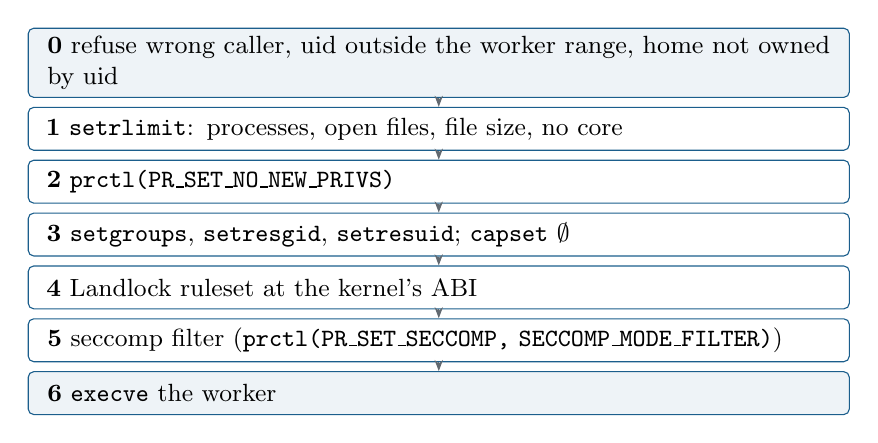
\begin{tikzpicture}[font=\small,
  st/.style={draw=accent,rounded corners=2pt,fill=white,minimum width=0.86\columnwidth,
             minimum height=1.55em,align=left,inner sep=3pt,text width=0.82\columnwidth},
  arr/.style={-{Stealth[length=4pt]},draw=ink!70}]
  \node[st,fill=soft] (a) {\textbf{0} refuse wrong caller, uid outside the worker range, home not owned by uid};
  \node[st,below=0.32em of a] (b) {\textbf{1} \code{setrlimit}: processes, open files, file size, no core};
  \node[st,below=0.32em of b] (c) {\textbf{2} \code{prctl(PR\_SET\_NO\_NEW\_PRIVS)}};
  \node[st,below=0.32em of c] (d) {\textbf{3} \code{setgroups}, \code{setresgid}, \code{setresuid}; \code{capset} $\emptyset$};
  \node[st,below=0.32em of d] (e) {\textbf{4} Landlock ruleset at the kernel's ABI};
  \node[st,below=0.32em of e] (f) {\textbf{5} seccomp filter (\code{prctl(PR\_SET\_SECCOMP, SECCOMP\_MODE\_FILTER)})};
  \node[st,below=0.32em of f,fill=soft] (g) {\textbf{6} \code{execve} the worker};
  \foreach \x/\y in {a/b,b/c,c/d,d/e,e/f,f/g} \draw[arr] (\x) -- (\y);
\end{tikzpicture}
\caption{The spawn helper's sequence. Each later step can only remove
access; nothing after step~3 can regain a privilege.}
\label{fig:layers}
\end{figure}

\code{no\_new\_privs} is what makes a capability-bearing binary safe to
leave on the worker's path: under it, an \code{exec} grants no file
capabilities, so a worker that runs the helper gains nothing. After the
uid switch the capability set is emptied, so no capability survives
into the worker. Landlock is applied after the switch and seccomp last,
so the helper's remaining work needs nothing the filter refuses. CPU
time is deliberately not limited by \code{RLIMIT\_CPU}, which counts a
process's whole life while workers are kept warm; each call is bounded
by the runtime's clock instead. Further subcommands chown, empty, and
sweep a uid's places, and \code{stop} kills every process of a uid, so
a browser never outlives the worker that started it.

\paragraph{One uid per approval}
Each approved agent gets a uid from a reserved range (one is reserved
for verifying packages, one for the builder). A worker's home is
emptied before every start, so it holds no state between starts.

\paragraph{Why not namespaces}
Inside a container's default profile a process cannot create user
namespaces; permitting it would mean relaxing the container's own
seccomp profile for everything in it. Separate uids, Landlock and a
seccomp filter provide the isolation without that cost.

\subsection{Files: Landlock}

The spawner names the paths; the helper hands them to the
kernel~\cite{landlock}. Read-and-execute: system directories, the
image's browsers, the agent's own package and environment. Read-write:
its home and spool. Write where ownership still decides: \code{/dev},
\code{/proc}, \code{/tmp}. Nothing else---not the platform's code,
other agents' packages, or the uid table. The helper validates none of
the paths: a Landlock ruleset can only remove access. The ruleset
requests what the running kernel supports (\cref{tab:landlock}). ABI~6
closes a channel that ownership and the firewall both miss: an abstract
Unix socket has a name but no inode, owner, or mode, and is invisible
to an address-based rule; from ABI~6 a fenced worker connects only to
abstract sockets created inside its own Landlock domain.

\begin{table}[t]
\centering\small
\caption{Landlock features requested by kernel ABI.}
\label{tab:landlock}
\begin{tabular}{@{}cll@{}}
\toprule
\textbf{ABI} & \textbf{Linux} & \textbf{Adds} \\
\midrule
1 & 5.13 & path-based file access \\
2 & 5.19 & \code{REFER}: moving files between own folders \\
3 & 6.2 & \code{TRUNCATE} \\
4 & 6.7 & TCP connect only to the proxy's port \\
6 & 6.12 & abstract Unix sockets scoped to own domain \\
\bottomrule
\end{tabular}
\end{table}

\subsection{System calls: seccomp}

The filter~\cite{seccomp} is a \emph{denylist}, on purpose: an agent may
bring any Python package, and an allowlist would be a list of what
somebody forgot. \Cref{tab:seccomp} shows what is refused for the
worker and all its descendants. \code{clone3} returns \code{ENOSYS}
rather than \code{EPERM}: its flags sit behind a pointer a BPF filter
cannot dereference, and glibc, told the call does not exist, falls back
to \code{clone}, whose flags the filter can inspect. Refusals return
the error codes programs already handle, so a package that probes a
call degrades instead of crashing. The filter is independent of the
container engine's profile and refuses what Docker's default allows,
\code{ptrace} among it. It is written so that the browser agents rely
on keeps working under it.

\begin{table}[t]
\centering\small
\caption{System calls refused to every worker.}
\label{tab:seccomp}
\begin{tabularx}{\columnwidth}{@{}>{\raggedright\arraybackslash}p{0.24\columnwidth}>{\raggedright\arraybackslash}X@{}}
\toprule
\textbf{Class} & \textbf{Calls} \\
\midrule
namespaces, mounts & \code{unshare}, \code{clone} with namespace flags, \code{setns}, \code{mount}, \code{umount2}, \code{pivot\_root}, the new mount API \\
cross-process memory & \code{ptrace}, \code{process\_vm\_readv/writev}, \code{pidfd\_getfd} \\
large kernel surface & \code{bpf}, \code{perf\_event\_open}, \code{userfaultfd}, \code{io\_uring\_*}, module and kexec loading, keyrings, \code{open\_by\_handle\_at} \\
socket families & all but \code{AF\_UNIX}, \code{AF\_INET}, \code{AF\_INET6}, and netlink for routes and device events \\
\bottomrule
\end{tabularx}
\end{table}

\subsection{Network: proxy, rule, hosts}

The egress proxy (\file{ai\_runtime/agents/egress.py}), running in the
runtime, (1)~identifies the worker by a per-worker pass and serves no
one else; (2)~refuses a host the manifest does not name; (3)~resolves
the name itself and refuses the host if \emph{any} answer is internal
(loopback, private, link-local---where cloud metadata lives), which
closes DNS rebinding toward the platform; and (4)~connects to the
address it checked and copies bytes. It terminates no TLS and installs
no certificate. Connections are bounded per worker and in total, and
every connection made or refused is recorded with its owner, host,
bytes each way, and duration. A host named by a credential or allowed
on a code card is \emph{lent} to the worker's pass only for the call.

The proxy is enforceable only because nothing else is reachable. At
container start, a root step installs an nftables rule on the output
hook matching the \emph{socket owner's uid} across the worker range:
accept TCP to one loopback port---the spawner's, which passes what
arrives to the runtime's proxy---and reject everything
else---other ports, other agents, the spawner, DNS. It then drops to
the platform's user with \code{net\_admin} removed from the bounding
set, so nothing started later can change the rule. Landlock's TCP rule
(ABI~4) is a second hold behind it.

\subsection{Dependencies: the builder}

A source distribution's build is arbitrary code. Installation is
therefore split: a dedicated \emph{builder} uid, under the same limits
and fences, whose proxy pass opens only the package index, downloads
and builds the declared requirements into wheels; one build at a time,
killed after five minutes, nothing persisting between builds. The
runtime then unpacks the wheels: it is handed files, never the list,
resolves and downloads nothing, and unpacking a wheel runs none of its
code.

\subsection{Memory}

A per-process address-space limit breaks browsers, so agents share a
memory budget. The spawner samples each agent's unique memory every
second and, at 90\% of the container's limit, ends the largest agent
with everything it runs, telling the affected call why.

\subsection{The inspector}

A sandbox one cannot see must be taken on faith. At every start,
before serving anyone, the platform tests its own locks: it starts a
process as an agent's user, asks the kernel which fences it can
enforce, prepares a place end to end, and tries to reach the network as
a worker would. It reports in plain words---\emph{workers are confined},
\emph{files are fenced}, \emph{system calls are filtered}---or which is
not, and why. If agents cannot be confined at all, the platform does not
start. If one lock is weaker on this machine (an older kernel without
Landlock, say), it runs, and every agent's page says what is not
enforced where it runs.

\section{Secrets and Data}
\label{sec:secrets}

\subsection{One shape for everything stored}

Credentials, agents' records, files, and skills (knowledge a person
writes for the assistant) are all one document type
(\code{ResourceStore}, \file{backend/database/stores/data/resources.py}),
so that the rules that matter are written once: a random reference; a
category; an \emph{owner map} of groups and people who may see it;
\emph{keys}, plain searchable facts (provider, account, expiry); and
\emph{values}, the sealed part (tokens, passwords). Keys can be listed
and searched; values cannot be searched at all.

\paragraph{Seeing is a filter, not a check}
Every read served to a caller is a single query carrying both the id
and the visibility filter
\[
\begin{array}{l}
\mathit{type}\ \land\ \mathit{org\_id} = o_r\ \land\\
\quad\bigl(\mathit{owner.groups} \cap G_r \neq \emptyset\ \lor\ r \in \mathit{owner.users}\bigr)
\end{array}
\]
for reader $r$ of organization $o_r$ with groups $G_r$ (including the
organization's Everyone sentinel). A check after a lookup is a line
somebody can forget; a filter inside the lookup is one they would have
to remove. A miss is the same 404 as a document that does not exist.

\paragraph{Seeing is not changing}
Each document has one steward, its creator, who alone may change,
share, transfer or delete it; a colleague it was shared with may use
it. Nobody may share beyond their reach: only into groups they belong
to and with people who share one. One named \emph{escape grant} per
kind lifts both rules for an administrator, and only over documents
the holder can already see.

\subsection{Encryption at rest}

Values are sealed with AES-256-GCM~\cite{nist80038d}
(\file{backend/database/crypto.py}). Keys are 32 bytes, versioned, used
as given with no derivation. Each encryption takes a fresh 96-bit
random nonce. The plaintext is the values map as compact JSON; the
\emph{associated data} is the document's id, so a sealed value copied
into another document does not open there (the owner is deliberately
not bound, since it changes on share and transfer). The stored form
records the algorithm and key version. Decryption fails closed on an
unknown algorithm, an unconfigured version, a failed tag, or a payload
that is not a JSON object, and never returns part of a map. Key
rotation adds a version, re-seals every stored value with a write
conditioned on the old version, and retires the old key only when
nothing is left under it. The same cipher seals model provider keys,
OAuth client secrets, repository tokens, and webhook secrets. Without
valid keys, the backend refuses to start; it never derives a key from
another setting. A credential's sealed half is never shown back to a
person under any permission.

\subsection{The path of a secret}

\begin{figure}[t]
\centering
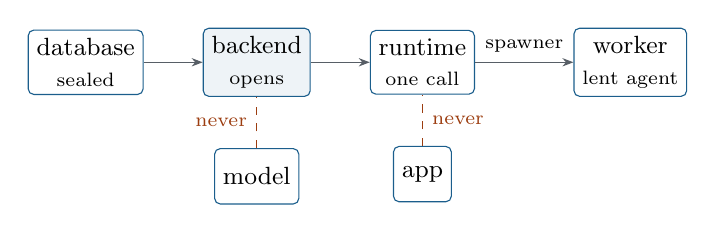
\begin{tikzpicture}[font=\small,
  n/.style={draw=accent,rounded corners=2pt,fill=white,align=center,inner sep=3pt,minimum height=2em},
  arr/.style={-{Stealth[length=4pt]},draw=ink!75},
  no/.style={draw=warn,dashed}]
  \node[n] (db) {database\\{\scriptsize sealed}};
  \node[n,right=0.75cm of db,fill=soft] (b) {backend\\{\scriptsize opens}};
  \node[n,right=0.75cm of b] (r) {runtime\\{\scriptsize one call}};
  \node[n,right=1.25cm of r] (w) {worker\\{\scriptsize lent agent}};
  \node[n,below=0.65cm of b] (m) {model};
  \node[n,below=0.65cm of r] (p) {app};
  \draw[arr] (db) -- (b);
  \draw[arr] (b) -- (r);
  \draw[arr] (r) -- node[above,font=\scriptsize]{spawner} (w);
  \draw[no] (m) -- node[left,font=\scriptsize,text=warn]{never} (b);
  \draw[no] (p) -- node[right,font=\scriptsize,text=warn]{never} (r);
\end{tikzpicture}
\caption{Where a decrypted secret exists. The spawner relays the line
unread. The model and the app never receive it.}
\label{fig:secret}
\end{figure}

A decrypted secret exists only in the backend, which opens it; the
runtime, which carries it for one call; and the worker of the agent it
was lent to (\cref{fig:secret}). The road, in order: the agent's code
asks for a declared secret; the runtime checks that the running
function declared \code{use} of it and maps the slot to
\code{<approval>\_\_<id>}; it calls the backend under the delegation;
the backend refuses any principal but the runtime, resolves the slot to
one credential (the chat's binding, the grant on the slot, the person's
default, or the only visible one---otherwise an error, never a guess),
re-reads it through the person's visibility filter, decrypts it,
appends \code{secret.use} to the audit trail (never the value), and
returns it. A host named by the credential is lent to the worker's
proxy pass until the call ends. The runtime keeps nothing past the call.

\paragraph{Connected accounts}
For OAuth credentials~\cite{rfc6749}, the platform---not the agent---runs
the authorization flow with PKCE~\cite{rfc7636}, keeps the tokens, and
refreshes them. At use, a token valid for more than another minute is
handed out with the refresh token removed; otherwise the backend
refreshes first. The refresh token and the organization's client secret
never leave the backend, so the worker receives only a short-lived
access token. A credential a person typed (an API key, a password)
reaches the worker as typed. On a phone, where the OAuth browser does
not carry the app's session, the callback parks the code behind a
one-use, two-minute hand-off that only the same person's app session
can redeem.

\paragraph{Lending}
Two agents may need the same account. A person can lend a credential to
another agent's slot only where the declared shapes match exactly and,
for a connected account, the provider and every declared scope match.
At use, the credential is re-read through the chatting person's filter,
so a lend gives nothing to someone who cannot see it.

\subsection{What a captured runtime could see}

The runtime holds no vault key and no database route. Through the
delegations it still holds, a runtime taken over could read what is
visible to those people---their credentials' access tokens
included---and nothing of anyone else's. It could not open a sealed
value itself or obtain a refresh token or client secret.

\section{Control and Accountability}
\label{sec:control}

\subsection{The clock}

Deferred work is written on the chat's clock rather than kept in the
model's mind (\file{ai\_runtime/chat/clock.py}). A row is either a
\emph{note}, which wakes the assistant at the set time as if the person
had written, or an \emph{unattended function}: one function with inputs
fixed when the row was made, run \emph{without the model}, waking the
assistant only when a named result field is non-empty. Only functions
the manifest marks \code{schedulable} may run this way, and that flag
is accepted only at level 0 or 1 without model use. At each fire the
chat's contract is re-read and the call passes every gate against what
the person is allowed \emph{that day}. A wake runs at the chat's trust
level like any turn: a send proposed on Friday waits on a card exactly
as Monday's did. Bounds: 50 rows per chat; repeating rows at least a
minute apart; a missed row fires once, never as a backlog.

\subsection{Stopping}

\paragraph{One chat}
\emph{Stop generating} asks the assistant to stop at the next point and
interrupts the call it awaits. \emph{Stop everything in this chat} is a
kill: the backend expires the chat's pending cards on the record, then
the runtime cancels the clock's fires under way, the assistant's cycle
and every job, and sends each worker call a protocol \code{cancel}; a
worker that does not answer within five seconds is killed with every
process of the agent's uid through the spawn helper. The chat's browser
is closed and its helpers ended. The runtime then records
\code{stopped} in the state so a rebuilt session rests, and saves.

\paragraph{Everything, and staying stopped}
The per-person switch acts in three steps (\code{Halt.stop},
\file{backend/api/services/chat\_session/halt.py}): (1)~mark the person
stopped, after which the backend neither dials nor mints a delegation
for them and their webhooks answer as if they did not exist;
(2)~kill every chat of theirs with a live delegation, schedule, or open
socket, concurrently, allowing ten seconds each; and (3)~delete every
delegation row. Because a delegation is accepted only while its row
exists, a program that ignored its order to end can no longer read a
credential, record, or file of the person's: the stop does not depend
on anything agreeing to stop. Only the person can resume; the switch
action is refused to runtime principals, so what is stopped cannot
restart itself.

\paragraph{Rules set beforehand}
Each organization has one Safety setting: sites no agent may open, how
often agent-written code is put to a person, which packages code may
install, whether MCP servers may be added and webhooks received, and
whether notifications may carry content or say only that something
happened.
Each rule is enforced where it can be: blocked sites at the proxy, code
rules in the backend as a card opens, the package list in the runtime
before a card, MCP and webhooks in the backend.

\subsection{The audit trail}

Nearly everything the platform lets happen leaves a line in an
append-only collection (\code{AuditStore},
\file{backend/database/stores/audit.py}), written at chokepoints by two
writers (\cref{tab:audit}). The runtime may write only lines of type
\code{execution}, so it cannot forge an approval or a credential read;
it does decide whether to write one. ``Append-only'' is a property of
the code, not the database: the store offers \code{append},
\code{search} and \code{for\_chat}; nothing calls an update or delete on
the collection, and no action exposes one. A line the database refuses
twice is written whole to the error log at \code{CRITICAL}, and the
action proceeds: auditing is a witness, not a gate. Each person may read
their own trail; the organization's trail is a separate grant.

\begin{table}[t]
\centering\small
\caption{Audit-trail writers.}
\label{tab:audit}
\begin{tabularx}{\columnwidth}{@{}>{\raggedright\arraybackslash}p{0.33\columnwidth}>{\raggedright\arraybackslash}X@{}}
\toprule
\textbf{Line} & \textbf{Writer and content} \\
\midrule
\code{execution} & runtime, per call: agent, function, declared and chat level, outcome, duration, inputs in outline, hosts reached \\
\code{approval.requested}, \code{.resolved} & backend, at the card \\
\code{secret.use}, \code{llm.use} & backend, where a credential or model key is served (reference only) \\
\code{agent.*}, \code{user.*}, \code{settings.safety}, \code{work.*}, \ldots & backend, at each controller \\
\code{webhook.received}, \code{.refused} & backend, at the webhook door (field names, never values) \\
\code{platform.action} & gateway: every non-read action outside the chat path, with outcome, never the payload \\
\bottomrule
\end{tabularx}
\end{table}

\subsection{The monitoring record}

The audit trail says what the platform \emph{allowed}. A second record,
kept beside the agents rather than in the database, says what agents'
programs \emph{did}: processes started and ended, log lines, and every
connection made or refused with host, resolved address, verdict, bytes,
and duration---never content. It is a bounded working log (128\,MiB,
oldest first), readable by administrators through dedicated grants.

\subsection{Notifications out}

A person may have their notifications sent to Slack, Teams, or a system
of their own. The platform posts a line and a link from a queue, so a
slow receiver delays nothing; it never sends a secret or the
conversation, and includes the reply text only on request. JSON
deliveries are signed with HMAC-SHA256~\cite{rfc2104} over
\code{"<timestamp>.<body>"}. An address must be HTTPS and resolve only
to public addresses, checked when subscribed and before each send;
redirects are not followed.

\section{Implementation}
\label{sec:implementation}

\sys{} is open source.\footnote{\url{https://github.com/decentai-io/decentai};
the public agent catalog is at
\url{https://github.com/decentai-io/decentai-agents}.} It is deployed
with Docker Compose as six services: Caddy (the single public entry,
also serving the web app), the backend, MongoDB, the runtime, the
agents' container, and a speech service. Three networks separate them
(\cref{fig:arch}): \code{default}, the only one with a route out;
\code{data}, internal, joining only the database, the backend, and a
one-shot initializer; and \code{agents}, internal, joining only the
runtime and the agents' container.

\begin{table}[t]
\centering\small
\caption{Implementation size (non-test source lines).}
\label{tab:loc}
\begin{tabular}{@{}lr@{}}
\toprule
\textbf{Component} & \textbf{Lines} \\
\midrule
Backend (Python, FastAPI) & 29{,}297 \\
Runtime and agents' container (Python) & 18{,}466 \\
Shared contracts: manifest, package, chat parts (Python) & 4{,}138 \\
Agent SDK (Python, standard library only) & 1{,}543 \\
Spawn helper (C) & 934 \\
Web app (TypeScript, Angular; \file{frontend/src/app}) & 33{,}717 \\
\bottomrule
\end{tabular}
\end{table}

\Cref{tab:loc} gives the size of each part. The backend owns identity,
policy, the data layer, encryption, OAuth, webhooks, and the audit
trail, behind one gateway. The runtime holds the assistant loop
(\file{ai\_runtime/mind/}), chat sessions and the clock
(\file{ai\_runtime/chat/}), the executor and resource mediation
(\file{ai\_runtime/execution/}), the worker pool and egress proxy
(\file{ai\_runtime/agents/}), and the spawner
(\file{ai\_runtime/agents\_container/}). Contracts shared by backend and
runtime---the manifest validator, the canonical package format, the
chat message parts---live in one package so the two sides cannot
disagree. Agent code imports only the SDK, which speaks the worker
protocol over standard input and output.

Model access goes through connectors for several provider protocols,
or a model served on the organization's own machines; the organization
configures connections and may scope keys per organization, group, or
person. A mobile client (Expo/React Native) is a thin remote control
for any instance: chat, approval cards, and notifications.

\section{Evaluation}
\label{sec:evaluation}

We evaluate whether the mechanisms hold as described, in three ways:
automated tests that exercise each promise the way a person, an agent,
or an attacker would (\cref{sec:eval-suites,sec:eval-hostile});
a structured analysis of what each adversary can reach
(\cref{sec:eval-analysis}); and a check that the documentation this
paper is built on matches the code (\cref{sec:eval-docs}). We close
with what is not evaluated (\cref{sec:eval-not}).

\subsection{Test suites}
\label{sec:eval-suites}

\Cref{tab:suites} summarizes the suites. Runtime tests run real agent
code in real processes, with a \emph{scripted model}: a stand-in that
returns replies written in advance. This is deliberate. The claims
under test concern what the \emph{platform} does with whatever the
model proposes (G1), and a test must give the same result on every run.
The runtime suite runs against in-memory services that answer the
backend's contract; the cross-component suite includes an end-to-end
test in which a person's socket reaches the backend, the backend dials
a real runtime process, and the runtime calls back through the gateway
under the chat's delegation, with nothing stubbed but the model.

\begin{table}[t]
\centering\small
\caption{Automated test suites (test functions; parametrization makes
the executed count higher). Results from runs on 15~October~2026.}
\label{tab:suites}
\begin{tabularx}{\columnwidth}{@{}>{\raggedright\arraybackslash}p{0.28\columnwidth}r>{\raggedright\arraybackslash}X@{}}
\toprule
\textbf{Suite} & \textbf{Tests} & \textbf{Exercises} \\
\midrule
Runtime & 1{,}031 & assistant loop, executor gates, approvals, clock, stops, proxy, evidence, documentation \\
Backend & 924 & identity, policy invariants, delegation fence, data layer and encryption, OAuth, webhooks, audit \\
Cross-component & 180 & approval-to-package path; end-to-end chat across backend and runtime \\
Example agent & 24 & an agent run as its author would \\
\midrule
\textbf{Total} & \textbf{2{,}159} & \\
\quad of which sandbox, live & 83 & hostile agent in the deployed two-container topology (\cref{sec:eval-hostile}) \\
\bottomrule
\end{tabularx}
\end{table}

\paragraph{Results}
On the main branch on 15~October~2026 (Python 3.11, MongoDB~7), every
suite passed with no failures: runtime, 1{,}056 passed and 85 skipped
(the 83 live sandbox tests, which need the Linux image and are reported
in \cref{sec:eval-hostile}, and two others); backend, 969 passed and 6
skipped; cross-component, 216 passed and 3 skipped; example agent, 24
passed. Executed counts exceed \cref{tab:suites} because of
parametrization.

\paragraph{Regression tests from review}
In October 2026 the entire code base was reviewed line by line. Every
case found to make the code fail, hang, or answer wrongly was fixed
together with a test that repeats the attempt; in the runtime these
are kept in dedicated ``edge'' files---around stops (26 tests), the
executor (17), contracts and the SDK (31), the clock (8), session
restarts (6), concurrent stores (8), reasoning budgets (14), and
services and connectors (24). Design questions the review raised but
did not settle are published with the code (\cref{sec:limitations}).

\subsection{Confinement against a hostile agent}
\label{sec:eval-hostile}

The way to test a lock is to try to open it. The live sandbox suites
(\file{ai\_runtime/tests/test\_confinement\_live.py},
\file{test\_spawner\_live.py}) install a fixture agent that is
\emph{hostile on purpose}: each of its functions attempts one escape,
and the test passes only when the attempt is refused. Beside each
refusal, positive controls check that legitimate work still functions,
since a sandbox that refuses everything would pass the first kind of
test and fail the second. A second hostile package attacks at
\emph{build} time, from a local package index.

\paragraph{Setup}
We ran both files in the deployed topology: the runtime's image as the
runtime, and again as the agents' container beside it on an internal
network, with \code{NET\_ADMIN} for the egress rule. The host kernel was
Linux 6.18 (WSL2), which offers every Landlock feature in
\cref{tab:landlock}, so no test was skipped for want of a kernel
feature.

\paragraph{Results}
All 83 tests passed and none was skipped (58 confinement tests and 25
tests of the spawner across the two containers; 88\,s wall time).
\Cref{tab:hostile} groups the attempts by the promise they test and
the layer that refuses them.

\begin{table*}[t]
\centering\small
\caption{Escape attempts by the hostile agent, each refused, and the
legitimate operations verified alongside. All 83 tests passed on Linux
6.18 with no skips.}
\label{tab:hostile}
\begin{tabularx}{\textwidth}{@{}>{\raggedright\arraybackslash}p{0.15\textwidth}>{\raggedright\arraybackslash}X>{\raggedright\arraybackslash}p{0.2\textwidth}>{\raggedright\arraybackslash}p{0.24\textwidth}@{}}
\toprule
\textbf{Promise} & \textbf{Attempts (all refused)} & \textbf{Refused by} & \textbf{Still works} \\
\midrule
P1 own files & read the runtime's settings; write into its own package, environment, or the install directory; read or write another agent's home or package; read the uid table or the platform's code; write where every user may write & uid ownership; Landlock & reads what it runs from; spool shared with the runtime; home emptied each start, even if closed or deeply nested \\
P2 own user & signal the runtime; use the spawn helper to become another agent's uid; close or deeply nest its home to keep state across restarts & uid separation; \code{no\_new\_privs}; empty capability set; the helper's \code{clear} & runs as its own uid in its own home; stopping it ends everything it started \\
P3 declared hosts & connect past the proxy; reach the runtime's own door or the spawner; resolve a name directly; reach an undeclared host; reach anything with \code{hosts: []} or no network block; reach a blocked site with \code{hosts: any} & nftables owner rule; proxy; Landlock TCP rule & reaches its declared host; a host its credential names, only for that call; a host a person allowed on a code card, only until the call ends \\
P4 bounded resources & (verified, not attacked) the worker finds on itself exactly the process, open-file and file-size limits the container set, never a manifest's & \code{setrlimit} & threads and subprocesses start \\
P5 system calls & open an unused socket family; \code{ptrace}; create a namespace; connect to another agent's abstract Unix socket & seccomp; Landlock scoping (ABI~6) & its own Unix socket; a program it runs is fenced with it \\
Builds & a hostile build reads settings, writes into the environment, reaches hosts other than the index, fetches packages from elsewhere, or never ends & builder uid; proxy pass; five-minute kill & wheels built and installed by the runtime; only wheels are left \\
Records & an agent reads the monitoring record & folder mode and Landlock & both containers write one record \\
\bottomrule
\end{tabularx}
\end{table*}

\subsection{Security analysis}
\label{sec:eval-analysis}

\Cref{tab:matrix} relates each adversary to what it can do and what
holds it. Two observations follow. First, the defences against A1 and
A2 are the same set of gates, and none of them reads model output: this
is what makes the design independent of whether injection is detected.
Second, the defences sit in components of different trust: compromising
a less trusted component (a worker, then the runtime) leaves in place
every defence held by a more trusted one---the backend's keys, its
database, its decision on approvals, and its ability to withdraw
delegations.

\begin{table*}[t]
\centering\small
\caption{Adversaries, their capabilities, and the mechanisms that hold them.}
\label{tab:matrix}
\begin{tabularx}{\textwidth}{@{}>{\raggedright\arraybackslash}p{0.15\textwidth}>{\raggedright\arraybackslash}p{0.27\textwidth}>{\raggedright\arraybackslash}X@{}}
\toprule
\textbf{Adversary} & \textbf{Can} & \textbf{Held by} \\
\midrule
A1 model & emit any action in the vocabulary, with any inputs; write any prose & every action validated and gated outside the model; grants deny by default; the level gate; evidence drawn only from the trace \\
A2 injector & choose text the model reads, and so steer its proposals & the same gates; none of grants, level, manifest hosts, approval hash or credential binding derives from model output; a denial refuses the named hosts to the whole agent for the rest of the request \\
A3 agent author & arbitrary code in the worker during a call & approval pinned to commit and digest; per-operation resource mediation; uid, Landlock, seccomp, limits; egress only to declared hosts; dependencies built by a separate confined user \\
A4 another person & their own session, cookie, or API key & sessions resolved per request; deny-by-default policy; reads filtered by visibility inside the query; tenant scoping; \code{Origin} check on cookie-bearing sockets \\
A5 compromised worker & the above, plus attacks on co-tenants of the container & sandbox layers; internal network leading only to the runtime \\
A6 compromised runtime & every delegation it currently holds & no database route, decryption key, or backend signing key; 40-action fence; cannot decide approvals; stop-everything withdraws its delegations \\
\bottomrule
\end{tabularx}
\end{table*}

\paragraph{Injection reach by trust level}
Because the gate is a single comparison, the reach of a successful
injection (A2) inside one chat can be stated exactly: a proposal runs
without a card if and only if the function is granted to the chat, its
inputs validate, its scopes fit the grant, and $\ell_f \le \ell_c$.
At the default $\ell_c = 1$, an injected proposal can at most read and
make ordinary changes through granted agents; every wider change and
every action leaving the platform becomes a card. At $\ell_c = 0$,
only reads run unasked. At $\ell_c = 3$, every granted function runs
unasked---the case the trust level exists to make a person's explicit
choice. In every case, egress remains restricted to declared hosts and
no credential is exposed to the model.

\paragraph{Blast radius}
A compromised worker holds what its call was handed, its own home, and
its declared hosts. A compromised runtime can act for the people whose
delegations it holds---people with a chat open or a schedule
running---within 40 actions, and, since the level gate runs in the
runtime, could run their granted functions without opening a card; it
cannot answer a card, read the database, open a sealed value, obtain a
refresh token, or act for anyone else. Delegations last at most an hour
and are withdrawn by the person's stop-everything switch. A
compromised backend is a compromise of the deployment; it is the one
component trusted with everything.

\subsection{Documentation held to the code}
\label{sec:eval-docs}

This paper is distilled from the project's documentation, which names
the files implementing each mechanism. Five tests hold that
documentation to the code: every relative link and heading anchor
resolves; every backticked repository path exists; every setting the
configuration page describes is read by code, and every setting the
example files offer is documented; and the published list of actions is
regenerated from the backend's catalog and must match. These tests
check what a page \emph{points at}; whether a sentence is true is for a
reader to verify, which is why each mechanism here names its file.

\subsection{What is not evaluated}
\label{sec:eval-not}

\begin{itemize}
\item \textbf{Model behaviour.} No test calls a real model. The tests
  show that a proposal cannot pass the gates; they do not measure
  whether a given model resists injected text or chooses well. Neither
  is a claim of this paper.
\item \textbf{Performance and scale.} We do not report latency or
  throughput overheads, nor behaviour with many organizations, chats,
  or concurrent fires.
\item \textbf{The kernel.} Confinement results hold on the kernel
  tested; a kernel flaw is a way past every layer, and no test rules one
  out.
\item \textbf{The web app's own tests} exist but were not part of this
  evaluation.
\end{itemize}

\section{Limitations}
\label{sec:limitations}

A security paper that lists only what works asks to be taken on faith.
We classify each known limit as \emph{chosen} (a trade-off made on
purpose), \emph{open} (raised by the October 2026 code review and not
yet decided; 137 such questions are published with the code, each
naming its file), or \emph{inherited} from the environment.

\paragraph{The model}
The platform does not make the model correct (\emph{chosen}). A yes is
only as good as the reading of the card. Injection still steers what
runs without a card at or below the chat's level, all granted functions
at level~3; there is deliberately no administrator ceiling on the level
(\emph{chosen}). A plan item counts as ``verified'' when it has
\emph{some} evidence: one successful call attaches to every active
item, and the model chooses which reference it cites (\emph{open}).

\paragraph{Agents and the sandbox}
An agent can misuse what it was rightly given: during a call it holds
the decrypted credential and may talk to its declared host, and the
proxy sees host and byte counts, never content (\emph{chosen}: reading
inside TLS would mean impersonating every site). Because workers are
kept warm, code that wants to could retain a credential beyond the
call---an OAuth access token until it expires, a typed key until it is
changed (\emph{chosen}; review before approval is the control). A
Google token carries every scope the catalog's Google agents share;
what keeps the Gmail agent to mail is its single declared host. The
kernel is shared by all containers (\emph{inherited}); the seccomp
filter exists only on x86-64 and arm64, and a deployment whose agents
need a refused call can switch it off---for every agent at once---both
stated at start. Two colluding
agents can exchange bytes through a file in \code{/tmp} or
\code{/dev/shm} on any kernel (\emph{open}), or through an abstract
socket before Linux 6.12 (\emph{inherited}). Once connected to a
declared address, an agent can ask that address for another site it
serves (\emph{open}). Memory is a shared pool sampled once a second, and
disk use is counted but not capped (\emph{chosen}).

\paragraph{People and organizations}
The sandbox separates agents, not the people who use one: one worker
per approved agent serves everyone in the organization granted it, so
its memory and a host lent for one person's call are shared with a
concurrent colleague's call (\emph{chosen}, for memory and start-up
cost). Tenants share the agents' container, so process listings and the
connection log span organizations, and an agent writing enough to its
error output can push others' connection records out of the bounded
log (\emph{open}); the audit trail is a separate store and unaffected.
A compromised runtime can act, within 40 actions and without opening
cards, for people whose delegations it holds (\emph{chosen}: a
scheduled chat must act while its person is away).

\paragraph{Data and records}
The audit trail is append-only by the code's shape, not by the
database: an operator with the database password could alter it
undetectably, as there is no hash chain (\emph{chosen}, consistent with
the out-of-scope operator). A call's inputs are recorded in outline as
proposed, so a password a person typed into the chat and the model
passed on, or a secret an agent placed in its error text, can reach the
trail (\emph{open}). An agent that returns a credential in its result
passes it to the model and the trail: results are validated for shape,
not scanned for secrets. File bytes are not sealed by the platform; they
rest on the backend's volume or in a cloud bucket encrypted by its
provider.

\paragraph{Webhooks}
Only \sys{}'s own signature scheme is verified; providers with their
own schemes are reached through a relay. The rate limit is counted per
backend process. An outbound address is checked by name and then
connected to by name, leaving a DNS-rebinding window (\emph{open}). An
event the chat could not receive is marked undelivered and not retried.

\paragraph{Operation}
One runtime serves a deployment, and nothing moves a chat between
runtimes (\emph{chosen}). A stop sent while a new message is being
prepared, which may include installing an agent, waits until that
preparation finishes; the per-person switch does not, since it
withdraws every delegation (\emph{open}). A one-off reminder whose fire
fails is spent without notice (\emph{open}). Agent code that writes to
standard output corrupts its own protocol line, and one blocking call
stalls a worker's other calls (\emph{open}); a broken worker fails
honestly and the next call starts a fresh one.

\section{Conclusion}
\label{sec:conclusion}

\sys{} takes the language model as it is---capable, fallible, and
steerable by what it reads---and builds around it a platform in which
the model holds no authority. Every proposed action meets gates whose
inputs are identity, grants, a person-chosen trust level, an agent's
approved manifest, and the person's approval of the exact call; none is
derived from model output. Untrusted agent code runs as its own user,
fenced by Landlock and seccomp, reaching only declared hosts through a
proxy, with credentials lent per call and never shown to the model.
What appears as data beside the model's words is drawn from stored,
validated results. A stop withdraws the keys rather than asking for
cooperation, and an append-only trail records what was allowed.

None of these mechanisms is new on its own; they are the protections
operating systems have offered programs for half a century. The
contribution is to place them around a planner that is very capable and
not trusted, so that when it is wrong---and it will be---the mistake is
contained to what a person could already do, visible on a card or in a
record, and stoppable. The implementation is open, the tests that hold
its claims can be rerun by anyone, and the limits are stated beside
them.

\section*{Acknowledgements}
AI tools (Claude, by Anthropic) assisted in drafting the text of this
paper and in checking its claims against the source code. The author
reviewed the text and is responsible for its content.

\section*{Availability}
The source code, documentation, and test suites are available at
\url{https://github.com/decentai-io/decentai}; the agent catalog used in
the examples is at \url{https://github.com/decentai-io/decentai-agents}.


\small
\bibliographystyle{plainnat}
\bibliography{references}

\end{document}
